\chapter{Chapter 6: Prototyping Embedded Devices}

This chapter compiles lecture-quality study notes and comprehensive exam answers for \textbf{Unit VI: Prototyping Embedded Devices} of the OE-EC803A syllabus, adhering strictly to the \textbf{MAKAUT Answer Writing Guidelines}.


\section{Section 1: Arduino vs. Raspberry Pi Platform Comparison (Q6.2) [5M]}

\subsection{1. Overview}
The \textbf{Arduino} and \textbf{Raspberry Pi} represent the two dominant paradigms in IoT prototyping hardware: the \textbf{microcontroller} (bare-metal, real-time, single-task) and the \textbf{microprocessor} (OS-based, multi-tasking, general-purpose computing).

\begin{figure}[H]
\centering
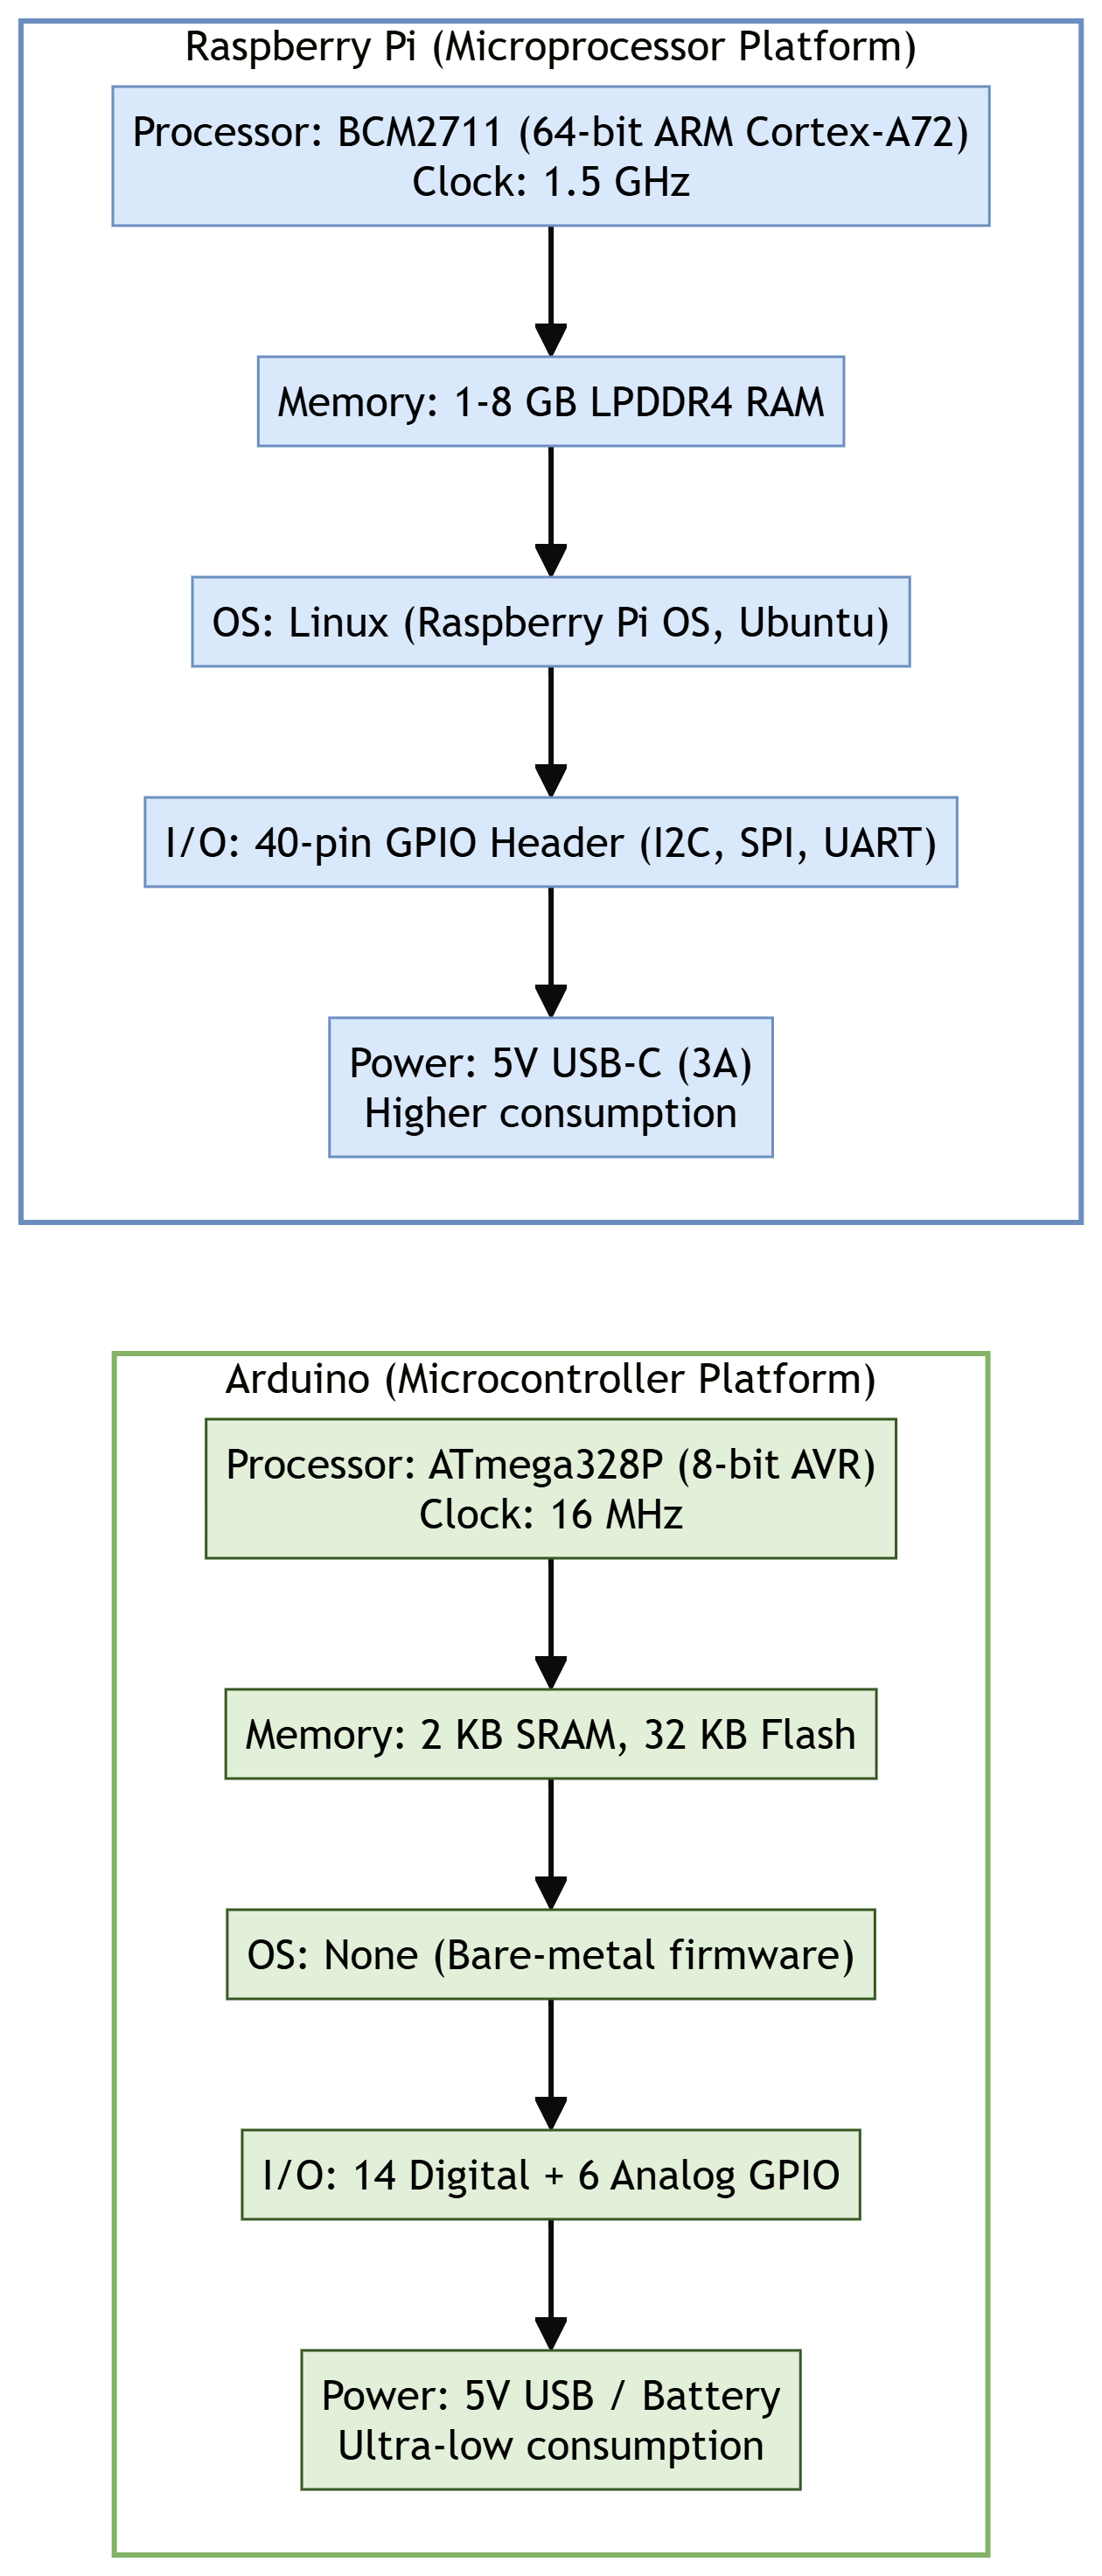
\includegraphics[width=0.75\textwidth,height=0.32\textheight,keepaspectratio]{../Images/chapter_06/arduino_vs_raspberry_pi.png}
\caption{Arduino vs. Raspberry Pi Architecture}
\end{figure}


\subsection{2. Detailed Feature Comparison}

\begin{table}[H]
\centering
\begin{tabular}{|p{\dimexpr 0.2\textwidth - 2\tabcolsep - 1.5\arrayrulewidth\relax}|p{\dimexpr 0.4\textwidth - 2\tabcolsep - 1.5\arrayrulewidth\relax}|p{\dimexpr 0.4\textwidth - 2\tabcolsep - 1.5\arrayrulewidth\relax}|}
\hline
Feature / Criteria & Arduino (e.g., Uno R3) & Raspberry Pi (e.g., Pi 4 Model B) \\
\hline
\textbf{Core Architecture} & 8-bit ATmega328P Microcontroller (AVR). & 64-bit BCM2711 Quad-core ARM Cortex-A72 Microprocessor (SoC). \\
\hline
\textbf{Clock Speed} & 16 MHz. & 1.5 GHz (nearly 100x faster). \\
\hline
\textbf{RAM} & 2 KB SRAM. & 1 GB to 8 GB LPDDR4. \\
\hline
\textbf{Flash/Storage} & 32 KB on-chip Flash. & MicroSD card (8 GB to 256 GB+). \\
\hline
\textbf{Operating System} & None (bare-metal firmware; code runs directly on the chip). & Full Linux distribution (Raspberry Pi OS, Ubuntu, Windows IoT Core). \\
\hline
\textbf{Programming Language} & C/C++ (via Arduino IDE). & Python, C/C++, Java, Node.js, and any Linux-supported language. \\
\hline
\textbf{I/O Capabilities} & 14 Digital I/O + 6 Analog Input pins. 10-bit ADC built-in. & 40-pin GPIO header (Digital only; no built-in ADC). Requires external ADC (e.g., MCP3008). \\
\hline
\textbf{Connectivity} & None on-board (requires external shields for Wi-Fi/BLE). & Built-in Wi-Fi (802.11ac), Bluetooth 5.0, Gigabit Ethernet, 2x USB 3.0. \\
\hline
\textbf{Power Consumption} & Ultra-low (~50 mA active). Can run on small batteries for months. & Higher (~600 mA to 1.2 A under load). Requires a stable 5V/3A USB-C supply. \\
\hline
\textbf{Boot Time} & Instant (microseconds; no OS to load). & 15–30 seconds (Linux kernel boot sequence). \\
\hline
\textbf{Target Application} & Real-time sensor reading, PWM motor control, dedicated single-task embedded loops. & Edge computing, image/video processing, running web servers, machine learning inference. \\
\hline
\end{tabular}
\end{table}


\subsection{3. Conclusion}
\begin{itemize}
  \item   Use \textbf{Arduino} when the project requires a single, deterministic, real-time control loop (e.g., reading a temperature sensor every 100 ms and triggering a relay).
  \item   Use \textbf{Raspberry Pi} when the project requires a full operating system, network stack, graphical processing, or complex multi-threaded logic (e.g., running an MQTT broker, hosting a web dashboard, or performing on-device machine learning).
\end{itemize}


\section{Section 2: Raspberry Pi Platform: Strengths, Limitations, and OS (Q6.3) [15M]}

\subsection{1. Introduction}
The \textbf{Raspberry Pi} is a credit-card-sized, single-board computer (SBC) developed by the Raspberry Pi Foundation. It features a powerful ARM-based System-on-Chip (SoC), full Linux operating system support, and a 40-pin GPIO header for hardware interfacing, making it one of the most versatile platforms for IoT prototyping.


\subsection{2. Strengths of Raspberry Pi in IoT (Minimum 5 Points)}
\begin{enumerate}
  \item \textbf{Full Operating System Support:} Runs complete Linux distributions, providing access to thousands of pre-built packages, libraries, and developer tools (e.g., Python pip packages, Node.js npm modules, Docker containers).
  \item \textbf{High Processing Power:} The quad-core ARM Cortex-A72 at 1.5 GHz can handle computationally intensive edge tasks like real-time video analysis (OpenCV), local speech recognition, and lightweight machine learning inference (TensorFlow Lite).
  \item \textbf{Rich Connectivity Stack:} Built-in dual-band Wi-Fi (2.4 GHz and 5 GHz), Bluetooth 5.0 (with BLE), and Gigabit Ethernet eliminate the need for external connectivity modules.
  \item \textbf{Extensive Community and Documentation:} Millions of tutorials, GitHub repositories, and active community forums ensure rapid troubleshooting and code reuse.
  \item \textbf{Versatile I/O via 40-pin GPIO Header:} Supports I2C, SPI, UART, and general-purpose digital I/O for direct sensor and actuator interfacing without additional microcontrollers.
  \item \textbf{Low Cost:} Priced between \$35 and \$75 (depending on RAM variant), making it accessible for students, hobbyists, and small-run commercial prototypes.
  \item \textbf{HDMI Output:} Allows direct connection to monitors for local dashboard displays, kiosk-mode applications, or digital signage.
\end{enumerate}


\subsection{3. Limitations of Raspberry Pi in IoT (Minimum 5 Points)}
\begin{enumerate}
  \item \textbf{No Built-in Analog-to-Digital Converter (ADC):} Cannot directly read analog sensors (e.g., potentiometers, LDRs). Requires external ADC chips like MCP3008 over SPI.
  \item \textbf{High Power Consumption:} Draws 600 mA to 1.2 A under load, making it unsuitable for battery-powered remote deployments without significant power management engineering.
  \item \textbf{Non-Real-Time Operating System:} Linux is a general-purpose OS with process scheduling and interrupts. It cannot guarantee deterministic, microsecond-level timing for critical real-time control loops (e.g., PID motor control).
  \item \textbf{SD Card Corruption Risk:} The operating system runs from a MicroSD card. Sudden power loss during a write operation can corrupt the filesystem, causing boot failures.
  \item \textbf{Thermal Throttling Under Sustained Load:} The BCM2711 SoC generates significant heat during sustained CPU-intensive tasks, causing automatic clock speed reduction (thermal throttling) unless a heatsink or active fan is installed.
  \item \textbf{Overkill for Simple Tasks:} Using a full Linux computer to blink an LED or read a single temperature sensor is wasteful in terms of cost, power, and complexity compared to a simple Arduino.
\end{enumerate}


\subsection{4. Supported Operating Systems}

\begin{table}[H]
\centering
\begin{tabular}{|p{\dimexpr 0.25\textwidth - 2\tabcolsep - 1.5\arrayrulewidth\relax}|p{\dimexpr 0.75\textwidth - 2\tabcolsep - 1.5\arrayrulewidth\relax}|}
\hline
Operating System & Description \\
\hline
\textbf{Raspberry Pi OS (formerly Raspbian)} & Official Debian-based Linux OS. Lightweight, optimized for Pi hardware. Available in Desktop (with GUI) and Lite (headless CLI) editions. \\
\hline
\textbf{Ubuntu Server / Desktop} & Canonical's official ARM64 builds. Ideal for server-grade IoT gateway applications and Docker container orchestration. \\
\hline
\textbf{Windows 10 IoT Core} & Microsoft's stripped-down Windows for ARM devices. Supports UWP (Universal Windows Platform) apps. No traditional desktop; headless or single-app kiosk mode. \\
\hline
\textbf{RISC OS} & A lightweight, non-Unix OS providing extremely fast boot times and low resource usage. Niche use. \\
\hline
\textbf{LibreELEC / OSMC} & Dedicated media center distributions based on Kodi. Used for smart display and digital signage IoT setups. \\
\hline
\textbf{RetroPie} & Retro gaming emulation distribution. Not directly IoT-relevant, but demonstrates the Pi's versatility. \\
\hline
\end{tabular}
\end{table}


\section{Section 3: GPIO Pin Mapping and Electrical Safety Rules (Q6.1) [5M]}

\subsection{1. What are GPIO Pins?}
\textbf{GPIO (General-Purpose Input/Output)} pins are programmable digital pins on the Raspberry Pi's 40-pin header that can be configured via software as either an \textbf{Input} (to read digital HIGH/LOW signals from sensors and switches) or an \textbf{Output} (to drive LEDs, relays, and other actuators).

\begin{figure}[H]
\centering
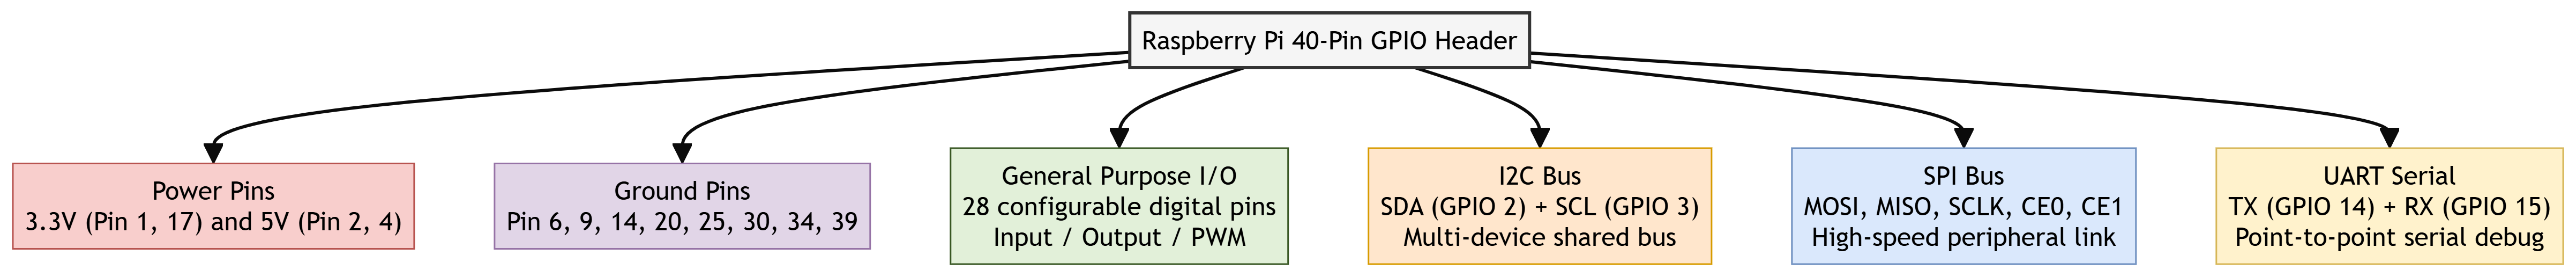
\includegraphics[width=0.75\textwidth,height=0.32\textheight,keepaspectratio]{../Images/chapter_06/rpi_gpio_interfaces.png}
\caption{Raspberry Pi GPIO Interfaces}
\end{figure}


\subsection{2. Communication Buses Available on the GPIO Header}
\begin{itemize}
  \item   \textbf{I2C (Inter-Integrated Circuit):} A shared, two-wire bus (SDA for data, SCL for clock) supporting multiple slave devices on the same bus via unique 7-bit addresses. Used for sensors like BMP280 (pressure) and OLED displays.
  \item   \textbf{SPI (Serial Peripheral Interface):} A high-speed, full-duplex, four-wire bus (MOSI, MISO, SCLK, CS). Used for high-throughput devices like external ADCs (MCP3008) and SD card modules.
  \item   \textbf{UART (Universal Asynchronous Receiver-Transmitter):} A simple, point-to-point serial link (TX and RX) at configurable baud rates. Primarily used for serial debugging consoles and communication with GPS modules.
\end{itemize}


\subsection{3. Five Critical Safety Guidelines for GPIO Pins}
Failure to follow these rules can permanently damage the Raspberry Pi's BCM2711 SoC:
\begin{enumerate}
  \item \textbf{Never Exceed 3.3V on Any GPIO Pin:} All GPIO pins are rated at 3.3V logic levels. Connecting a 5V signal directly will destroy the pin's internal ESD protection diodes.
  \item \textbf{Never Draw More Than 16 mA Per Pin:} Each GPIO pin can safely source or sink a maximum of 16 mA. To drive high-current loads (motors, relays), use an external transistor (e.g., 2N2222) or a MOSFET driver.
  \item \textbf{Never Short 5V to 3.3V or GND:} Accidentally shorting the 5V power rail (Pin 2/4) to any 3.3V GPIO pin or GND will create a direct short circuit through the voltage regulator, potentially frying the board.
  \item \textbf{Always Use Current-Limiting Resistors:} When driving LEDs, always place a series resistor (e.g., $330\ \Omega$) to limit current below the 16 mA pin rating.
  \item \textbf{Never Connect or Disconnect Wires While Powered On (Hot-Plugging):} Always shut down the Pi and disconnect power before modifying the wiring on the GPIO header to prevent accidental shorts.
\end{enumerate}


\section{Section 4: Alternative Prototyping Platforms (Q6.4) [10M]}

\subsection{1. BeagleBone Black}

\subsubsection{Overview:}
The \textbf{BeagleBone Black} is an open-source, community-supported single-board computer manufactured by Texas Instruments. It is positioned as a more industrial-grade alternative to the Raspberry Pi.

\subsubsection{Key Characteristics:}
\begin{itemize}
  \item   \textbf{Processor:} AM3358 ARM Cortex-A8 (1 GHz, 32-bit).
  \item   \textbf{Memory:} 512 MB DDR3 RAM + 4 GB on-board eMMC flash storage.
  \item   \textbf{GPIO:} 2 × 46-pin expansion headers providing \textbf{65 digital I/O pins}, 7 analog inputs (built-in 12-bit ADC), 4 timers, and 8 PWM outputs.
  \item   \textbf{OS:} Debian Linux (pre-installed on eMMC), Ubuntu, and Android.
\end{itemize}

\subsubsection{Strengths:}
\begin{enumerate}
  \item \textbf{Built-in ADC:} Unlike the Raspberry Pi, it has native analog input capability (7 channels at 1.8V max).
  \item \textbf{PRU (Programmable Real-Time Units):} Two independent 200 MHz real-time co-processors that can handle deterministic, microsecond-level I/O tasks alongside the main Linux OS.
  \item \textbf{On-board eMMC:} Avoids SD card corruption issues; boots from internal flash.
\end{enumerate}

\subsubsection{Limitations:}
\begin{enumerate}
  \item Smaller community and fewer tutorials compared to Raspberry Pi.
  \item Lower CPU performance than the Pi 4 (single-core Cortex-A8 vs. quad-core Cortex-A72).
\end{enumerate}


\subsection{2. Electric Imp}

\subsubsection{Overview:}
The \textbf{Electric Imp} is a proprietary, cloud-connected IoT development platform designed for rapid commercial product deployment. It is unique because it tightly integrates hardware, software, and a managed cloud backend into a single, vendor-controlled ecosystem.

\subsubsection{Key Characteristics:}
\begin{itemize}
  \item   \textbf{Hardware Module:} A small, Wi-Fi-enabled microcontroller module (imp001, imp004m, imp006).
  \item   \textbf{Programming:} Uses a proprietary language called \textbf{Squirrel} (a lightweight, C-like scripting language).
  \item   \textbf{Architecture:} All device logic is split into two parts:
  \item   \textbf{Device Code (Agent):} Runs on the physical module.
  \item   \textbf{Cloud Code (Server):} Runs on Electric Imp's managed cloud servers.
  \item   \textbf{Security:} End-to-end hardware-verified TLS encryption from chip to cloud.
\end{itemize}

\subsubsection{Strengths:}
\begin{enumerate}
  \item \textbf{Zero-Configuration Security:} Hardware-level authentication eliminates the need for manual key management.
  \item \textbf{Rapid Cloud Integration:} Devices automatically connect to the vendor's cloud on boot, reducing backend infrastructure setup time.
  \item \textbf{Production-Ready:} Pre-certified modules (FCC/CE) accelerate the path from prototype to manufactured product.
\end{enumerate}

\subsubsection{Limitations:}
\begin{enumerate}
  \item \textbf{Complete Vendor Lock-In:} If Electric Imp discontinues its cloud service, all connected devices become non-functional.
  \item \textbf{Proprietary Language:} Squirrel has a tiny community and minimal third-party library support.
  \item \textbf{Recurring Cloud Costs:} Requires ongoing subscription fees for the managed cloud backend.
\end{enumerate}


\subsection{3. Mobile Phones and Tablets as IoT Platforms}

\subsubsection{Overview:}
Modern smartphones and tablets are powerful IoT development platforms due to their rich built-in sensor arrays and ubiquitous connectivity.

\subsubsection{Key Characteristics:}
\begin{itemize}
  \item   \textbf{Built-in Sensors:} Accelerometer, gyroscope, magnetometer, barometer, ambient light sensor, proximity sensor, GPS, camera, microphone.
  \item   \textbf{Connectivity:} Wi-Fi, BLE, NFC, Cellular (4G/5G).
  \item   \textbf{Processing:} Multi-core ARM processors with GPUs capable of on-device machine learning inference.
\end{itemize}

\subsubsection{Strengths:}
\begin{enumerate}
  \item Eliminates the need to source, solder, and assemble individual sensor breakout boards.
  \item Pre-built user interfaces (touchscreen) for rapid app prototyping.
  \item Massive developer ecosystems (Android SDK, iOS Swift).
\end{enumerate}

\subsubsection{Limitations:}
\begin{enumerate}
  \item High power consumption and large physical form factor compared to dedicated embedded boards.
  \item Not designed for always-on, unattended operation (battery drain, OS updates, thermal shutdowns).
  \item Limited direct GPIO access for custom hardware interfacing.
\end{enumerate}


\subsection{4. Plug Computing (Always-On IoT)}

\subsubsection{Overview:}
A \textbf{Plug Computer} is a small, low-power, wall-socket-mounted computing device designed for always-on, unattended network services. It draws power directly from the wall outlet, eliminating battery concerns entirely.

\subsubsection{Key Characteristics:}
\begin{itemize}
  \item   \textbf{Form Factor:} Shaped like a large wall charger or power adapter.
  \item   \textbf{Example Devices:} SheevaPlug, DreamPlug, GuruPlug.
  \item   \textbf{Processor:} ARM-based (e.g., Marvell Kirkwood 1.2 GHz).
  \item   \textbf{OS:} Runs standard Linux distributions.
  \item   \textbf{Connectivity:} Gigabit Ethernet, Wi-Fi, USB host ports.
\end{itemize}

\subsubsection{Strengths:}
\begin{enumerate}
  \item \textbf{Always-On by Design:} Powered directly from mains electricity; ideal for 24/7 home automation hubs, NAS (Network Attached Storage), or local MQTT brokers.
  \item \textbf{Extremely Small Footprint:} Occupies only a wall socket; no desk space or wiring clutter.
  \item \textbf{Silent Operation:} No fans or moving parts; passively cooled.
\end{enumerate}

\subsubsection{Limitations:}
\begin{enumerate}
  \item \textbf{Very Limited GPIO:} Typically only USB and Ethernet ports; no direct sensor/actuator interfacing without USB-to-GPIO adapters.
  \item \textbf{Thermal Constraints:} Small enclosed form factor limits heat dissipation, restricting sustained CPU-intensive workloads.
  \item \textbf{Declining Market Availability:} Many original plug computer manufacturers have discontinued their products.
\end{enumerate}
